

%*** General probabilistic notation ***

\newcommand{\expv}{\mathbf{E}} % EXP. VALUE
\newcommand{\discProbDist}{f} % Discrete prob distribution
\newcommand{\sampleSpace}{S} % Generic sample space
\newcommand{\sigmaAlg}{\mathcal{F}} % Generic sigma-algebra
\newcommand{\probm}{\mathbb{P}} % Generic probability measure, also prob. measure operator
\newcommand{\rvar}{X} % Generic random variable
%\newcommand{\dist}{\mathit{Dist}}

%*** MDP notation ***

\newcommand{\actions}{A} % The set of actions.
\newcommand{\colouring}{c} % the colouring function
\newcommand{\probTranFunc}{\Delta} % Transition function of an MDP
\newcommand{\edges}{E} % Set of edges in an MDP.
\newcommand{\colours}{C} % The set of colours in an MDP.
\newcommand{\mdp}{\mathcal{M}} % A generic MDP. 
\newcommand{\vinit}{v_0} % An initial vertex in an MDP.
\newcommand{\cylProb}{p} % Function assigning probabilities to cylinder sets in 
%the measure construction.
\newcommand{\emptyPlay}{\epsilon} %empty play
\newcommand{\objective}{\Omega} % Qualitative objective
\newcommand{\genColour}{\textsc{c}} % Generic colour
\newcommand{\quantObj}{f} % Generic quantitative objective
\newcommand{\indicator}[1]{\mathbf{1}_{#1}} % In.d RV
\newcommand{\eps}{\varepsilon} % Numerical epsilon
\newcommand{\maxc}{W} % Maximal abs. value of a colour

\newcommand{\winPos}{W_{>0}}
\newcommand{\winAS}{W_{=1}}
\newcommand{\cylinder}{\mathit{Cyl}}

\newcommand{\PrePos}{\text{Pre}_{>0}}
\newcommand{\PreAS}{\text{Pre}_{=1}}

\newcommand{\PreOPPos}{\mathcal{P}_{>0}}
\newcommand{\OPAS}{\mathcal{P}_{=1}}

\newcommand{\safeOP}{\mathit{Safe_{=1}}}
\newcommand{\closed}{\mathit{Cl}}

\newcommand{\reachOP}{\mathcal{V}}
\newcommand{\discOP}{\mathcal{D}}
\newcommand{\valsigma}{\vec{x}^{\sigma}}

\newcommand{\lp}{\mathcal{L}}
\newcommand{\lpdisc}{\lp_{\mathit{disc}}}
\newcommand{\lpmp}{\lp_{\mathit{mp}}}
\newcommand{\lpsol}[1]{\bar{#1}}
\newcommand{\lpmpdual}{\lpmp^{\mathit{dual}}}

\newcommand{\actevent}[3]{\actions^{#1}_{#2,#3}} % Returns #1-th action on the run 

\newcommand{\MeanPayoffSup}{\MeanPayoff^{+}}
\newcommand{\MeanPayoffInf}{\MeanPayoff^{-}}

\newcommand{\mcprob}{M}
\newcommand{\invdist}{\vec{z}}

\newcommand{\hittime}{T}



A possible taxonomy of algorithms for solving parity games distinguishes three families:
\begin{itemize}
	\item ``strategy improvement algorithms'', which construct a sequence of improving strategies until reaching an optimal strategy. 
	We will construct in \cref{3-sec:strategy_improvement} an exponential time strategy improvement algorithm.
	
	\item ``attractor decomposition algorithms'', which decompose a game through a sequence of attractor computations. 
	The first and archetypical example is McNaughton Zielonka algorithm defined in \cref{2-sec:parity}. 
	We will present in \cref{3-sec:zielonka} a quasipolynomial time algorithm improving over this algorithm.

	\item ``value iteration algorithms'', which find an optimal strategy through the computation of a value function.
	An equivalent point of view on this family of algorithms is the use of separating automata for reducing parity games to safety games.
	We introduce the framework of separating automata in \cref{3-sec:separation} and give a quasipolynomial time algorithm as an instanciation of it. 
	We then construct value iteration algorithms through the notion of universal trees in \cref{3-sec:value_iteration},
	and present a third quasipolynomial time algorithm in the form of a value iteration algorithm.
\end{itemize}

As a conclusion \cref{3-sec:relationships} discusses the relationships between the different algorithms: in what sense are separating automata and value iteration algorithms equivalent through the notion of universal trees, and how does this family compare to the other two families of algorithms described above.

\begin{remark}
We already proved in \cref{2-thm:parity} that parity games are positionally determined for both players, so in this chapter when considering a strategy we implicitly assume that it is positional.
\end{remark}

%%%%%%%%%%%%%%%%%%
%%%%%%%%%%%%%%%%%%
%%%%%%%%%%%%%%%%%%

\section{An exponential time strategy improvement algorithm}
\label{3-sec:strategy_improvement}
Value iteration algorithms manipulate value functions and never construct any strategy, at least explicitly.
This is a key difference with strategy improvement algorithms (also called policy iteration algorithms) whose fundamental idea is to maintain and improve a strategy.
We assume that the games we consider in this section are positionally determined, therefore all strategies are assumed to be positional.

\vskip1em
Let us consider a game $\game$ and set as a goal to construct an optimal strategy for Eve.
As for value iteration algorithms we work with a value function: 
the key idea behind strategy improvement is to use $\val^{\sigma}$ to improve the strategy $\sigma$ 
by \emph{switching} an edge, which is an operation that creates a new strategy.
This involves defining the notion of \emph{switchable edge}:
the edge $(v,u)$ is switchable if 
\[
\delta(\val^{\sigma}(u),\col(v)) > \delta(\val^{\sigma}(v'),\col(v)) \text{ where } \sigma(v) = (v,v').
\]
Intuitively: according to $\val^{\sigma}$, playing $(v,u)$ is better than playing $\sigma(v)$.

Given a strategy $\sigma$ and an edge $e = (v,u)$ we use $\sigma[v \to e]$ to denote the strategy playing $e$ from $v$ and all other vertices follow $\sigma$.
Let us write $\sigma \le \sigma'$ if for all vertices $v$ we have $\val^{\sigma}(v) \le \val^{\sigma'}(v)$,
and $\sigma < \sigma'$ if additionally $\neg (\sigma' \le \sigma)$.

The difficulty is that $e = (v,u)$ being switchable does not mean that it is a better move than $\sigma(v)$ in any context,
but only according to the value function $\val^{\sigma}$, so it is not clear that $\sigma[v \to e]$ is better than $\sigma$.
Strategy improvement algorithms depend on the following two principles.

\begin{property}[Progress]
\label{1-property:progress}
Let $\sigma$ be a strategy and let $e = (v,u)$ be a switchable edge. 
Then $\sigma < \sigma[v \to e]$.
\end{property}

\begin{property}[Optimality]
\label{1-property:optimality}
Let $\sigma$ be a strategy that has no switchable edges, then $\sigma$ is optimal.
\end{property}

The algorithm is the following: start at an initial strategy $\sigma_0$. 
In each round $i$ compute $\val^{\sigma_i}$ and look for a switchable edge.
If there exists a switchable edge $e_i = (v_i,v'_i)$, let $\sigma_{i+1} = \sigma_i[v_i \to e_i]$ and iterate to the next round.
Otherwise, return the optimal strategy $\sigma_i$.

The algorithm computes a sequence of strategies 
$\sigma_0 < \sigma_1 < \sigma_2 < \dots$.
Note that any such sequence must be finite, since at each step we strictly increase in the ordering and there are only finitely many (positional) strategies. 

\vskip1em
If both progress and optimality principles hold as stated this yields a strategy improvement algorithm computing the optimal strategy.
Unfortunately such ideal properties rarely hold and it is often necessary to state and prove weaker properties,
we refer to \cref{3-chap:parity,4-chap:payoffs} for examples.
%Let us illustrate this by looking at \cref{1-fig:counter_example_strategy_improvement} representing a CoB{\"u}chi game.
%Assume that the initial strategy is $\sigma_0$ defined by 
%$\sigma_0(v_0) = (v_0,v_1),
%\sigma_0(v_1) = (v_1,v_1)$,
%and $\sigma_0(v_2) = (v_2,v_1)$.
%This strategy is losing from all vertices since it eventually ends up looping around $v_1$.
%This implies that there are no switchable edges and in particular the two winning self loops around $v_0$ and $v_1$ are not considered.
%However $\sigma_0$ is clearly not optimal, contradicting the progress principle.
%
%For this reason the initial strategy $\sigma_0$ must be carefully chosen.
%A solution is to add for each vertex of Eve a new edge for stopping the game, 
%and to define $\sigma_0$ to be the strategy choosing this option from every vertex.
%The benefit of this approach is to avoid declaring some vertices losing only because they are losing with the (badly chosen) initial strategy.
%
%\begin{figure}
%\centering
%  \begin{tikzpicture}[scale=1.3]
%    \node[s-eve] (v0) at (0,0) {$\begin{array}{c} v_0 \\ 2 \end{array}$};
%    \node[s-eve] (v1) at (2,0) {$\begin{array}{c} v_1 \\ 3 \end{array}$};
%    \node[s-eve] (v2) at (4,0) {$\begin{array}{c} v_2 \\ 2 \end{array}$};
%    % create edges
%    \path[arrow]
%      (v1) edge[bend left] (v0)
%      (v0) edge[bend left] (v1)
%      (v1) edge[bend left] (v2)
%      (v1) edge[selfloop=90] (v1)
%      (v2) edge[bend left] (v1)
%      (v2) edge[selfloop=0] (v2)
%      (v0) edge[selfloop=180] (v0);
%  \end{tikzpicture}
%\caption{The optimality principle rarely holds, here illustrated on a CoB{\"u}chi game.}
%\label{1-fig:counter_example_strategy_improvement}
%\end{figure}

\begin{remark}
In the description above we did not specify which switchable edge to choose.
Actually strategy improvement algorithms often switch more than one edge at a time, making this question worse: 
which subset of the switchable edges should be chosen? 
Many possible rules for choosing this set have been studied, as for instance the \emph{greedy all-switches} rule. 
\end{remark}


%%%%%%%%%%%%%%%%%%
%%%%%%%%%%%%%%%%%%
%%%%%%%%%%%%%%%%%%

\section{A quasipolynomial time attractor decomposition algorithm}
\label{3-sec:zielonka}
\input{zielonka}

%%%%%%%%%%%%%%%%%%
%%%%%%%%%%%%%%%%%%
%%%%%%%%%%%%%%%%%%

\section{A quasipolynomial time separating automata algorithm}
\label{3-sec:separation}
\subsection*{The separation framework}
We describe a general approach for reducing parity games to safety games.
\Cref{1-sec:reductions} constructs reductions between objectives using automata: 
in the case at hand parity reduces to safety if there exists a deterministic automaton $\Automaton$ over the alphabet $[1,d]$
with acceptance objective $\Safe$ and defining $\Parity([1,d])$,
meaning $L(\Automaton) = \Parity([1,d])$.
With such an automaton in hand~\cref{1-lem:automata_reduction} implies the following reduction:
from a parity game $\game$ construct the safety game $\game \times \Automaton$ satisfying that
Eve has a winning strategy in $\Game$ from $v_0$ if and only if she has a winning strategy in $\Game \times \Automaton$ from $(v_0,q_0)$.

\vskip1em
Unfortunately, it can be shown (using a topological argument) that there is no such automaton.
The separation framework defines a (weaker) sufficient condition for the reduction above to be correct.
Instead of insisting that $L(\Automaton) = \Parity([1,d])$,
it is enough to have $\WE(\arena,\Parity[\col]) = \WE(\arena,L(\Automaton)[\col])$.
To ensure this equality we will only require that $L(\Automaton)$ \textit{separates} winning plays from losing plays.
The two \textit{key} ideas are first to take advantage of the positionality of parity objectives 
by restricting further winning plays to \textit{positional} winning plays,
and second to state $\WE(\arena,\Parity[\col]) = \WE(\arena,L(\Automaton)[\col])$ not for all parity games,
but only for parity games with $n$ vertices and priorities in $[1,d]$.

\vskip1em
A deterministic safety automaton over the alphabet $[1,d]$ is given by 
\[
\Automaton = (Q,q_0,\delta : Q \times [1,d] \to Q,\Safe[\col_\Automaton]),
\]
where $\col_\Automaton : Q \times [1,d] \to \set{\Win,\Lose}$.
A word $w \in [1,d]^\omega$ is accepted if the run $\rho$ over $w$ only contains transitions in $\Win$.
We use the following simplifying convention for safety automata: we distinguish a special rejecting state $\bot$
and assume that all transitions are accepting except the ones leading to $\bot$. 
Said differently, a word $w$ is accepted if and only if it the run over $w$ does not contain the state $\bot$.
Hence we do not need to specify $\col_\Automaton$:
in the next two sections by an automaton we mean a deterministic safety automaton
given by $\Automaton = (Q,q_0,\delta : Q \times [1,d] \to Q)$.

\vskip1em
Let us now give a sufficient condition for the automaton $\Automaton$ 
to imply the correctness of the reduction from the parity game $\Game$ to the safety game $\Game \times \Automaton$.
The condition that we define now is that the automaton $\Automaton$ is $(n,d)$-separating; it relies on the notion of parity graphs.
Recall a parity graph ""satisfies"" parity from $v$ if all infinite paths from $v$ satisfy parity,
and that a strategy $\sigma$ is winning from $v$ if and only if the parity graph $\Game[\sigma]$ satisfies parity from $v$.

We say that an automaton reads, accepts, or rejects a path $\pi$ in a parity graph, 
which is an abuse because what the automaton reads is the induced sequence of colours $\col(\pi)$.

\begin{definition}[Separating automata]
\label{3-def:separating_automata}
An automaton $\Automaton$ is $(n,d)$-\textit{separating} if the two following properties hold.
\begin{itemize}
	\item For all parity graphs $G$ with $n$ vertices and priorities in $[1,d]$ satisfying parity from $v$, 
	all paths from $v$ are accepted by $\Automaton$.
	
	\item All words accepted by $\Automaton$ satisfy parity.
\end{itemize}
\end{definition}
We define the objective $\Parity_{\mid n}$ over the set of colours $[1,d]$ as:
\[
\Parity_{\mid n} = 
\set{ \play : 
\begin{array}{l}
\play \text{ is a path starting from some vertex $v$ in some parity graph} \\
\text{with } n \text{ vertices and priorities in } [1,d] \text{ satisfying } \Parity \text{ from } v
\end{array}}.
\]
%For a parity graph $G$ and a vertex $v$, we let $\Paths(G,v) \subseteq [1,d]^\omega$ denote the set of infinite paths from $v$.
%We define the objective $\Parity_{\mid n}$ over the set of colours $[1,d]$ as:
%\[
%\Parity_{\mid n} = \bigcup \set{ \Paths(G,v) : 
%\begin{array}{l}
%G \text{ parity graph with } n \text{ vertices and priorities in } [1,d] \\
%\text{ satisfying } \Parity \text{ from } v
%\end{array}}.
%\]
The definition of $(n,d)$-separating automata is illustrated in \cref{3-fig:separation} and can be summarised
as $\Parity_{\mid n} \subseteq L(\Automaton) \subseteq \Parity$.

\begin{figure}[!ht]
\centering
  \begin{tikzpicture}
    \begin{scope}
      \draw[clip,use as bounding box] (0,0) ellipse (2cm and 1.2cm);
      \draw[dgrey] (0,0) ellipse (2cm and 1.2cm);
      \draw[white] (-2,0) ellipse (2.9cm and 2.5cm);
      \draw[lgrey] (-2,0) ellipse (1.5cm and 1.3cm);
      \draw[hatcharea,hatchspread=6pt] (-2,0) ellipse (2.1cm and 1.7cm);
      \draw (0,0) ellipse (2cm and 1.2cm);
    \end{scope}
    \path[arrow]
      (2.2,1.6) node[] {$[1,d]^\omega \setminus$ \textsf{Parity}} edge (1.5,.3)
      (0,1.6) node[] {\textsf{Parity}} edge (.4,.5)
      (-2,1.6) node[] {\textsf{Parity}$_{|n}$} edge (-1.4,.2)
      (-1.5,-1.5) node[below,anchor=base] {$L(\Automaton)$} edge (-.4,-.6);
  \end{tikzpicture}
\caption{The separation problem.}
\label{3-fig:separation}
\end{figure}

The following lemma shows the definition of separating automata in action.

\begin{lemma}[Game equivalence using separating automata]
\label{3-lem:separating_automata}
Let $\Automaton$ an $(n,d)$-separating automaton.
Then for all parity games $\game = (\arena,\Parity[\col])$ with $n$ vertices and priorities in $[1,d]$, 
we have
\[
\WE(\game) = \WE(\arena,L(\Automaton)[\col]).
\]
\end{lemma}

\begin{proof}
The inclusion $\WE(\game) \subseteq \WE(\arena,L(\Automaton)[\col])$ follows from positional determinacy and the inclusion 
$\Parity_{\mid n} \subseteq L(\Automaton)$.
Let $v \in \WE(\game)$.
Consider $\sigma$ a positional strategy ensuring parity from $v$ and construct the parity graph $\game[\sigma]$, it satisfies parity from $v$.
Hence the strategy $\sigma$ also ensures $L(\Automaton)[\col]$ from $v$, so $v \in \WE(\arena,L(\Automaton)[\col])$.

Conversely, the inclusion $L(\Automaton) \subseteq \Parity$ implies the inclusion 
$L(\Automaton)[\col] \subseteq \Parity[\col]$, which in turn implies 
$\WE(\arena,L(\Automaton)[\col]) \subseteq \WE(\game)$.
\end{proof}

The last step is to explain how to solve a game with objective $L(\Automaton)$, as already discussed in~\cref{1-sec:reductions}.
Let $\Game = (\arena, L(\Automaton)[\col])$.
We construct a safety game by making the synchronised product of the arena with the automaton:
\[
\Game \times \Automaton = (\arena \times \Automaton, \Safe[\col']),
\]
where the safety condition ensures that the play is accepted by $\Automaton$.
Formally, we construct the arena $\arena \times \Automaton$ as follows.
We first define the graph $G \times Q$ whose set of vertices is $V \times Q$ and set of edges is defined as follows:
for every edge $(v,v') \in E$ and state $q \in Q$ there is an edge from $(v,q)$ to $(v',\delta(q,\col(u)))$.
The arena is $\arena \times \Automaton = (G \times Q, \VE \times Q, \VA \times Q)$.
Using the convention for safety automata that the rejecting transitions are precisely those leading to the rejecting state $\bot$,
the colouring function is defined by $\col'(v,q) = \Win$ if $q \neq \bot$, and $\Lose$ otherwise.

\begin{fact}[Reduction to safety games using separating automata]
\label{3-fact:reduction}
Eve has a winning strategy in $\game$ from $v_0$ if and only if
she has a winning strategy in $\Game \times \Automaton$ from $(v_0,q_0)$.
\end{fact}

\begin{theorem}[Algorithm using separating automata]
\label{3-thm:algorithm_separating_automata}
Let $\Automaton$ an $(n,d)$-separating automaton.
There exists an algorithm for solving parity games of complexity $O(m \cdot |\Automaton|)$.
\end{theorem}
\begin{proof}
Let $\Game$ a parity game with $n$ vertices and priorities in $[1,d]$.
Thanks to~\cref{3-lem:separating_automata} and \cref{3-fact:reduction}, solving $\Game$
is equivalent to solving the safety game $\Game \times \Automaton$.
Thanks to~\cref{2-thm:reachability} solving safety games can be done in time linear in the number of edges.
This yields an algorithm for solving parity games whose running time is $O(m \cdot |\Automaton|)$.
\end{proof}

In the remainder of this section we give a construction for a quasipolynomial $(n,d)$-separating automaton.

\subsection*{The original separating automaton}
\begin{theorem}[The original separating automaton]
\label{3-thm:original_separating_automaton}
There exists an $(n,d)$-separating automaton of size $n^{O(\log d)}$,
inducing an algorithm for solving parity games of complexity $n^{O(\log d)}$.
\end{theorem}

\paragraph{\bf $i$-sequences.}
The key definition used by the original separating automaton is an
\emph{$i$-sequence}. Let $\pi = p_1, p_2, \dots, p_t$ a finite sequence of
priorities. An $i$-sequence is a set of \emph{indices} that splits $\pi$ into
sub-sequences. An $i$-sequence consists of exactly $2^i$ indices $1 \le j_1 <
j_2 < \dots < j_{2^i} \le t$, where each $j_k$ is an integer that refers to the
priority $p_{j_k}$ from the sequence $\pi$. An $i$-sequence is required to
satisfy the following properties. 
\begin{itemize} \item \textbf{Evenness.} Each
index (except possibly the last index) refers to an even priority, meaning that
$p_{j_k}$ is an even priority for all $k < 2^i$.

\item \textbf{Inner domination.} The subsequence of priorities between any two
indices $j_k$ and $j_{k+1}$ is dominated by either $p_{j_k}$ or $p_{j_{k+1}}$.
Formally, this means that whenever $j_k < l < j_{k+1}$, we have that $p_l \le
p_{j_k}$ or we have that $p_l \le p_{j_{k+1}}$.

\item \textbf{Outer domination.} The final subsequence between $p_{j_{2^i}}$ and
$p_t$ is dominated by $p_{j_{2^i}}$, meaning that for all $l > j_{2^i}$ we have
$p_l \le p_{j_{2^i}}$.
\end{itemize}

\begin{figure}[!ht]
    \begin{center}
    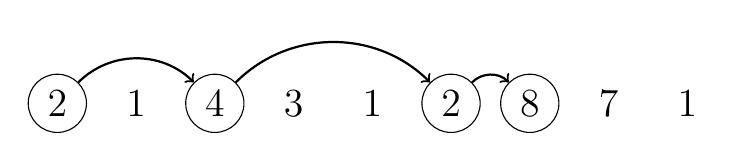
\begin{tikzpicture}

    \tikzstyle{seqc}=[draw, circle]

    \node [seqc] (1) {\Large $2$};
    \node [right of=1, node distance=1cm] (2) {\Large $1$};
    \node [seqc, right of=2, node distance=1cm] (3) {\Large $4$};
    \node [right of=3, node distance=1cm] (4) {\Large $3$};
    \node [right of=4, node distance=1cm] (5) {\Large $1$};
    \node [seqc, right of=5, node distance=1cm] (6) {\Large $2$};
    \node [seqc, right of=6, node distance=1cm] (7) {\Large $8$};
    \node [right of=7, node distance=1cm] (8) {\Large $7$};
    \node [right of=8, node distance=1cm] (9) {\Large $1$};

    \path[->,thick,bend left=45]
        (1) edge (3)
        (3) edge (6)
        (6) edge (7)
        ;
    \end{tikzpicture}
    \end{center}
    \caption{A $2$-sequence.}
\label{3-fig:isequence}
\end{figure}

\Cref{3-fig:isequence} gives an example of a $2$-sequence. The circled
priorities are the indices used in the sequence. Note that there are exactly
$2^2 = 4$ indices used, and that every circled priority is even. Inner
domination is satisfied because every priority that is between two circled
priorities is lower than one of the two end points, and outer domination is
satisfied because the final circled priority $8$ is larger than all the
priorities that come after it.

\paragraph{\bf The relationship to parity games.}
The relationship between $i$-sequences and parity games is explained by the
following lemma.

\begin{lemma}[Completeness for the separating automaton]
\label{3-lem:isequencewin}
Suppose that Adam and Eve play positional strategies in the parity game,
and let $\pi$ the resulting play.
\begin{itemize}
\item If Eve wins the parity game, then there exists prefixes of $\pi$ that
contain arbitrarily long $i$-sequences.
\item If Adam wins the parity game, then no prefix of $\pi$ will contain a
$\lceil \log n \rceil$-sequence.
\end{itemize}
\end{lemma}
\begin{proof}
If Eve wins the parity game then the largest
priority occurring in $\pi$ infinitely often is even. Let $p$ this priority.
To construct a prefix containing an $i$-sequence, we find the first index $j$
after which no priority $q > p$ is seen. We take as our indices $j_1 < j_2 <
\dots < j_{2^i}$ the first $2^i$ occurrences of priority $p$ after index $j$.
Evenness is trivially satisfied, and both inner and outer domination are
satisfied because no priority larger than $p$ is seen after index $j$.

We prove the second claim by contradiction. Suppose that Adam wins the game, but
that there is a prefix of $\pi$ that contains a $\lceil \log n \rceil$-sequence.
Since the sequence indexes $2^{\lceil \log n \rceil} \ge n$ vertices of the
game, it must index the same vertex $v$ twice. Thus our $i$-sequence must
contain a cycle passing through $v$. Note that inner domination ensures that the
largest priority on the cycle that passes through $v$ is even. However, no even
cycle can be formed when Adam wins the game by playing a positional winning
strategy, and so we have arrived at our contradiction.
\end{proof}

To summarise, if Eve wins the game, then she has a strategy that ensures that
arbitrarily long $i$-sequences occur, while if Adam wins the game then he has a
strategy that ensures that no $\lceil \log n \rceil$-sequence occurs. So to
solve the parity game, it is sufficient to determine whether Eve can force a
$\lceil \log n \rceil$-sequence to occur.

\paragraph{\bf A data structure for recognising $i$-sequences.}
We will build a quasi-polynomial sized automaton that reads a sequence of
priorities, 
and determines whether that sequence of priorities contains a
$k$-sequence. 
The automaton is defined by a data structure that we call a \emph{record}, which
contains information about the $i$-sequences that have been seen so far in the
sequence.  

A record is a sequence $b_k, b_{k-1}, \dots, b_1, b_0$, where each
$b_i$ is either a priority, or the special symbol $\siblank$. The value of $b_i$
has the following meaning: 
\begin{itemize}
\item \textbf{Witnessing.} If $b_i \ne \siblank$, then we have seen an
$i$-sequence, and the final priority on that $i$-sequence is $b_i$. 
\item \textbf{Order.} If $b_i \ne \siblank$ and $b_j \ne \siblank$ and $j < i$,
then the first index of the $j$-sequence witnessed by $b_j$ occurs after the
last index of the $i$-sequence witnessed by $b_i$.
\end{itemize}
Note that, although each element $b_i$ records the existence of an
$i$-sequence, the record data structure \emph{does not} store the $2^i$ indices
of this $i$-sequence, it only stores the priority of the final index of that
sequence.

\begin{figure}[!ht]
    \begin{center}
    \begin{tikzpicture}
    \tikzstyle{seqc}=[draw, circle]
    \node [seqc,red] (1) {\Large $2$};
    \node [right of=1, node distance=0.9cm] (2) {\Large $1$};
    \node [seqc, red, right of=2, node distance=0.9cm] (3) {\Large $4$};
    \node [seqc, red, right of=3, node distance=0.9cm] (4) {\Large $2$};
    \node [seqc, red, right of=4, node distance=0.9cm] (5) {\Large $8$};
    \node [right of=5, node distance=0.9cm] (6) {\Large $7$};
    \node [seqc, blue, right of=6, node distance=0.9cm] (7) {\Large $2$};
    \node [right of=7, node distance=0.9cm] (8) {\Large $1$};
    \node [seqc, blue, right of=8, node distance=0.9cm] (9) {\Large $4$};
    \node [right of=9, node distance=0.9cm] (10) {\Large $1$};
    \node [seqc, grey, right of=10, node distance=0.9cm] (11) {\Large $2$};

    \path[->,thick,bend left=45,red]
        (1) edge (3)
        (3) edge (4)
        (4) edge (5)
        ;

    \path[->,thick,bend left=45,blue]
        (7) edge (9)
        ;
    \end{tikzpicture}
    \end{center}
\caption{An example sequence that corresponds to the record $\siblank 8 4 2$.}
\label{3-fig:ds}
\end{figure}

\Cref{3-fig:ds} shows an example sequence that is consistent with the
record that sets $b_3 = \siblank$, $b_2 = 8$, $b_1 = 4$, and $b_0 = 2$.
The red $2$-sequence is represented by $b_2 = 8$, which is the last priority of
the $2$-sequence. The blue $1$-sequence starts after the end of the
$2$-sequence, and it is represented by $b_1 = 4$. Likewise the grey
$0$-sequence starts after the end of the $1$-sequence, and is represented by
$b_0 = 2$. There is no $3$-sequence in the example, and this is represented by
setting $b_3 = \siblank$.

\paragraph{\bf The update rule.}
Suppose that we have a record that represents the $i$-sequences in a
finite sequence of priorities, and that we then read the next priority $p$ in
that sequence. We need to update the record to take this priority into
account. We do this by applying the following \emph{update rule}.
The update rule consists of two steps, which occur one after the other.

\begin{itemize}
\item \textbf{Step 1.} In this step, we find the largest index $i$
such that $b_j$ is even for all $j \le i$. If $b_i = \siblank$, or $b_i < p$,
then we create a new record $b'_k$, $b'_{k-1}$, \dots, $b'_0$ by
setting:
\begin{equation*}
b'_j = \begin{cases}
b_j & \text{if $j > i$,} \\
p & \text{if $j = i$,} \\
\siblank & \text{if $j < i$.} 
\end{cases}
\end{equation*}
If there is no index $i$ that satisfies the conditions, then we do not modify
the record.

\item \textbf{Step 2.} In step 2, we take the output of step 1, and we find the
largest index $i$ such that $p > b_i$ and we create a new record $b'_k$,
$b'_{k-1}$, \dots, $b'_0$ by setting:
\begin{equation*}
b'_j = \begin{cases}
b_j & \text{if $j > i$,} \\
p & \text{if $j = i$,} \\
\siblank & \text{if $j < i$.} 
\end{cases}
\end{equation*}
Again, if there is no such index $i$, then the record is not modified.
\end{itemize}

\begin{figure}[!ht]
    \begin{center}
    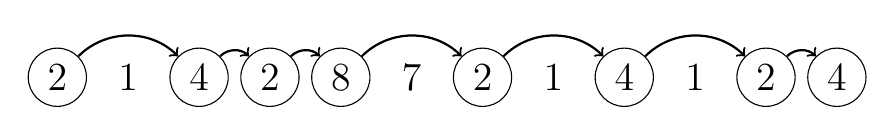
\begin{tikzpicture}
    \tikzstyle{seqc}=[draw, circle]
    \node [seqc] (1) {\Large $2$};
    \node [right of=1, node distance=0.9cm] (2) {\Large $1$};
    \node [seqc, right of=2, node distance=0.9cm] (3) {\Large $4$};
    \node [seqc, right of=3, node distance=0.9cm] (4) {\Large $2$};
    \node [seqc, right of=4, node distance=0.9cm] (5) {\Large $8$};
    \node [right of=5, node distance=0.9cm] (6) {\Large $7$};
    \node [seqc, right of=6, node distance=0.9cm] (7) {\Large $2$};
    \node [right of=7, node distance=0.9cm] (8) {\Large $1$};
    \node [seqc, right of=8, node distance=0.9cm] (9) {\Large $4$};
    \node [right of=9, node distance=0.9cm] (10) {\Large $1$};
    \node [seqc, right of=10, node distance=0.9cm] (11) {\Large $2$};
    \node [seqc, right of=11, node distance=0.9cm] (12) {\Large $4$};
    %\onslide<5>{\node [seq, right of=11, node distance=0.9cm] (12) {\Large
    %$\mathbf{9}$};}

    \path[->,thick,bend left=45]
        (1) edge (3)
        (3) edge (4)
        (4) edge (5)
        (5) edge (7)
        (7) edge (9)
        (9) edge (11)
        (11) edge (12)
        ;

    \end{tikzpicture}
    \end{center}
    \caption{An example of a Step 1 update applied to the sequence and record from~\cref{3-fig:ds}}
\label{3-fig:ds1}
\end{figure}
Intuitively, Step 1 attempts to combine the $i$-sequences in the existing record
into a longer $i$-sequence. Suppose that we have read the sequence shown in~\cref{3-fig:ds}, 
that we have compute the record $\siblank 8 4 2$, and that the next priority in the sequence is $4$.
\Cref{3-fig:ds1} shows the result of applying Step 1 to this situation.
Observe that $3$ is the largest index $i$ such that for all $j < i$ we have that
$b_j$ is even, so Step 1 will output the record $4 \siblank \siblank \siblank$.

So in this circumstance, Step 1 claims that we have now seen a $3$-sequence.
\Cref{3-fig:ds1} shows why this is correct: the $0$-sequence of $b_0$, the
$1$-sequence of $b_1$, and the $2$-sequence of $b_2$ can be merged together,
along with the new priority, to create a $3$-sequence. Observe that inner
domination in this new $3$-sequence is satisfied due to the outer domination
property for each of the $i$-sequences that it was constructed from.
For example, the $2$-sequence ends at priority $8$, and the $1$-sequence begins
at priority $2$, and we know that $8$ must dominate all priorities between the
$8$ and the $2$ because $8$ is required to dominate \emph{all} priorities that
follow it.

\begin{figure}[!ht]
    \begin{center}
    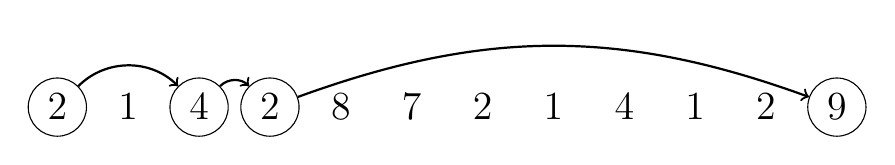
\begin{tikzpicture}
    \tikzstyle{seqc}=[draw, circle]
    \node [seqc] (1) {\Large $2$};
    \node [right of=1, node distance=0.9cm] (2) {\Large $1$};
    \node [seqc, right of=2, node distance=0.9cm] (3) {\Large $4$};
    \node [seqc, right of=3, node distance=0.9cm] (4) {\Large $2$};
    \node [right of=4, node distance=0.9cm] (5) {\Large $8$};
    \node [right of=5, node distance=0.9cm] (6) {\Large $7$};
    \node [right of=6, node distance=0.9cm] (7) {\Large $2$};
    \node [right of=7, node distance=0.9cm] (8) {\Large $1$};
    \node [right of=8, node distance=0.9cm] (9) {\Large $4$};
    \node [right of=9, node distance=0.9cm] (10) {\Large $1$};
    \node [right of=10, node distance=0.9cm] (11) {\Large $2$};
    \node [seqc, right of=11, node distance=0.9cm] (12) {\Large $9$};
    %\onslide<5>{\node [seq, right of=11, node distance=0.9cm] (12) {\Large
    %$\mathbf{9}$};}

    \path[->,thick,bend left=45]
        (1) edge (3)
        (3) edge (4);

    \path[->,thick,bend left=20]
        (4) edge (12)
        %(5) edge (7)
        %(7) edge (9)
        %(9) edge (11)
        %(11) edge (12)
        ;

    \end{tikzpicture}
    \end{center}
    \caption{An example of a Step 2 update applied to the sequence and record from~\cref{3-fig:ds}}
\label{3-fig:ds2}
\end{figure}

Step 2 ensures that the outer domination property holds. 
In~\cref{3-fig:ds2}, we show the result of applying Step 2 to the record
$\siblank 8 4 2$ that corresponds to the sequence shown in~\cref{3-fig:ds},
when the next priority in the sequence is $9$. Observe that since $9 > 8$, the
outer domination property for the $2$-sequence ending at $8$ now fails to hold,
and likewise for the sequences ending at $4$ and $2$. Hence, Step 2 deletes the
$0$-sequence and $1$-sequence from the record, and updates the $2$-sequence to
end at $9$, thereby restoring outer domination. The resulting record is $\siblank
9 \siblank \siblank$.

\paragraph{\bf Correctness.} 
To compute a record for a particular sequence of priorities, we start with the
record $\siblank \siblank \dots \siblank$, and then process the sequence one
priority at a time, using the update rule that we have described. 

We must now argue that the record data structure and update rule is sufficient
to decide the winner of a parity game. The following lemma states that a record
will never falsely claim that an $i$-sequence has occurred.

\begin{lemma}[Correctness for the separating automaton]
\label{3-lem:correctness_separating_automata}
Let $b_k, b_{k-1}, \dots, b_0$ the record for a sequence of priorities $\pi$.
If $b_i \ne \siblank$, then $\pi$ contains an $i$-sequence.
\end{lemma}
\begin{proof}
This can be proved by induction over the components of the record. In fact we
will prove the slightly stronger order property that we mentioned earlier:
the $i$-sequence corresponding to
$b_i$ starts after the $j$ sequence corresponding to $b_j$ whenever $i < j$ and
$b_i \ne \siblank$ and $b_j \ne \siblank$.

The base case is trivially true, since the value of $b_0$ asserts the existence
of a 0-sequence, and any priority by itself is a $0$-sequence. So when Step 1 or
Step 2 updates $b_0$, the corresponding $0$-sequence is the new priority, and
this clearly starts after all other $i$-sequences in the record.

For the inductive step, we must prove that the two steps of the update rule are
correct. 
\begin{itemize}
\item For Step 1 updates, we can use the inductive hypothesis to argue that, for
each $j < i$, the $j$-sequence corresponding to $b_j$ exists, and that they
appear in order in the sequence, and that it ends before the sequence
corresponding to $b_{j-1}$ starts. Furthermore, the outer domination property
the $j$-sequence ensures that all priorities between the end of the
$j$-sequence and the start of the $(j-1)$-sequence are dominated by the last
priority in the $j$-sequence, which must be even according to the definition of
a Step 1 update.
Hence, we can combine all of the $j$-sequences with $j < i$ together, along with
the new priority, to create an $i$-sequence. This new $i$-sequence starts at
exactly the same point as the sequence corresponding to $b_{i-1}$, and so the
order property still holds.

\item For Step 2 updates, we only need to argue that the value of $b'_i$
correspond to an $i$ sequence. This can be constructed as we showed in~\cref{3-fig:ds2}: 
take the $i$-sequence that corresponds to $b_i$, and
replace the final priority with the new priority. Observe that the final
priority of an $i$-sequence is permitted to be odd, and so this new sequence
satisfies all of the requirements of an $i$-sequence. Furthermore, the starting
point of this sequence has not changed, and so the order property is preserved.
\end{itemize}
\end{proof}

As a consequence of the lemma above, if Adam has a strategy to ensure that no
$k$-sequence occurs in the game, then Adam has a strategy to ensure that the
$b_k$ component of the record is never set so that $b_k \ne \siblank$.

It can be shown that the other direction is also true: if an $i$-sequence has
occurred, then there will be some index $j \ge i$ such that $b_j \ne \siblank$.
However, the proof is somewhat tedious, and this statement is actually stronger
than what we need. To argue that the record can determine the winner of a parity
game, the following weaker lemma suffices. 

\begin{lemma}[Weaker correctness for the separating automaton]
\label{3-lem:weaker_correctness_separating_automaton}
Let $\pi$ an infinite play that is winning for Eve. For all $k$, there exists
a prefix of $\pi$ such that $b_k \ne \siblank$.
\end{lemma}
\begin{proof}
Let $p$ the largest even priority that is seen infinitely often, and let $j$
be the first index after which no priority larger than $p$ is visited. We argue
that after index $j$ has been reached, the record will eventually set $b_i \ne
\siblank$ for all $i$.

To see why, observe that after index $j$ has been reached, Step 2 cannot replace
any component $b_j$ with $b_j = p$, since Step 2 can only overwrite the priority
in $b_j$ when the new priority $p'$ satisfies $p' > b_j$, but no priority $p' >
p$ is seen after index~$j$. 

On the other hand, Step 1 will always be triggered whenever we visit the
priority $p$. Step 1 will always set some component of the record to $p$, and as
we have observed this cannot be overwritten by Step 2. Moreover, since $p$ is
even, repeated application of Step 1 will
build a longer and longer $i$-sequences whose outer domination
priority is $p$. Thus, after we have made $2^k$ visits to $p$, we will have set
$b_k = p \ne \siblank$, if we have not done so already.
\end{proof}

Hence, if Eve wins the parity game, then she has a strategy to eventually ensure
that $b_k \ne \siblank$. Combining the two lemmas above, with~\cref{3-lem:isequencewin} gives the following corollary.

\begin{corollary}[Correctness of the reduction for the separating automaton]
\label{3-cor:correctness_reduction_separating_automaton}
Suppose that we monitor the play of a parity game with a record $b_{\lceil \log
n \rceil}, \dots, b_0$. Eve has a strategy that ensures $b_{\lceil \log n
\rceil} \ne \siblank$ if and only if Eve wins the parity game.
\end{corollary}

\paragraph{\bf The size of the automaton.}
The record data structure and update rule can be encoded as a deterministic
finite automaton that reads the play. Each state of the automaton is associated
with some configuration of $b_{\lceil \log n \rceil}, \dots, b_0$, and the
transitions of the automaton are defined by the update rule. 

This automaton has quasipolynomial size. The number of states used in the
automaton is the number of possible configurations of
$b_{\lceil \log n \rceil}, \dots, b_0$. Each $b_i$ can be one of the $d$
priorities in the game, or the symbol $\siblank$, and so there are $d + 1$
possible values that it can take. Moreover there are $\log n + 1$ components of
the record, so the total number of configurations is at most
$(d+1)^{\log n +1} = n^{O(\log d)}$.



%%%%%%%%%%%%%%%%%%
%%%%%%%%%%%%%%%%%%
%%%%%%%%%%%%%%%%%%

\section{A quasipolynomial time value iteration algorithm}
\label{3-sec:value_iteration}
\begin{theorem}
\label{3-thm:value_iteration_quasipoly}
There exists a value iteration algorithm for solving parity games in time 
\[
O\left(nm \log(n) \log(d) \cdot  \binom{\lceil \log(n) \rceil + d/2 - 1}{\lceil \log(n) \rceil} \right),
\]
which is quasipolynomial in general and polynomial if $d = O(\log(n))$.
The space complexity of the algorithm is $O(m + n \log(d))$.
\end{theorem}

We rely on the high-level presentation of value iteration algorithms given in \cref{1-sec:value_iteration}.
Let $\game = (\arena,\Parity[\col])$ a parity game with $n$ vertices and priorities in $[1,d]$,
and without loss of generality $d$ is even.

The first step is to define a notion of value function $\val^\game : V \to Y$ with $(Y,\le)$ a lattice satisfying the characterisation principle:
for all vertices $v$ we have that Eve wins from $v$ if and only if $\val^\game(v) \neq \bot$, where $\bot$ is the least element in $Y$.
The goal of the algorithm is to compute $\val^\game$, from which we then easily obtain the winning region thanks to the characterisation principle.

To set the machinery of value iteration algorithms in motion we can either construct $\val^\game$ as the unique fixed point of a contracting operator using Banach's fixed point theorem or the greatest fixed point of a monotonic operator using Kleene's fixed point theorem.

Let us here follow the second approach. 
We let $F_V$ be the lattice of functions $V \to Y$ equipped with the componentwise order induced by $Y$.
We are looking for a monotonic function $\delta : Y \times [1,d] \to Y$ inducing the operator $\Op : F_V \to F_V$ defined by:
\[
\Op(\mu)(v) = 
\begin{cases}
\max \set{\delta( \mu(v'), \col(v)) : (v,v') \in E} & \text{ if } v \in \VE, \\
\min \set{\delta( \mu(v'), \col(v)) : (v,v') \in E} & \text{ if } v \in \VA,
\end{cases}
\]
such that $\val^\game$ is the greatest fixed point of $\Op$.
The algorithm would then simply use \cref{1-thm:kleene} to compute $\val^\game$ by iterating the operator $\Op$.

Let us look at this question using the notion of progress measures, which are post-fixed points of $\Op$,
meaning $\mu$ such that $\mu \le \Op(\mu)$. 
Since the greatest fixed point of $\Op$ is also its greatest post-fixed point, an equivalent formulation of the characterisation principle above reads: for all vertices $v$ we have that Eve wins from $v$ if and only if there exists a progress measure $\mu$ such that $\mu(v) \neq \bot$.

To summarise this discussion, we are looking for a lattice $(Y,\le)$ and a monotonic function $\delta : Y \times [1,d] \to Y$ 
such that for all parity games $\Game$ with $n$ vertices and priorities in $[1,d]$, 
for all vertices $v$ we have that Eve wins from $v$ if and only if there exists a progress measure $\mu$ such that $\mu(v) \neq \bot$.
Our next step is to show how the notion of universal trees provides a class of solutions to this problem.
%\footnote{One can even show that any solution is equivalent to a universal tree, but we will not prove it in this chapter.}

\subsubsection*{Universal trees}
The trees we consider have three properties: 
they are rooted, every leaf has the same depth, and the children of a node are totally ordered.
Formally, a tree of height $0$ is a leaf,
and a tree $t$ of height $h + 1$ is an ordered list $[t_1,\dots,t_k]$ of subtrees each of height $h$.

We consider two parameters for trees: the height, and the size which is defined to be the number of branches (equivalently, the number of leaves).
All trees we consider have height $h = d/2$.

\begin{figure*}[!ht]
\centering
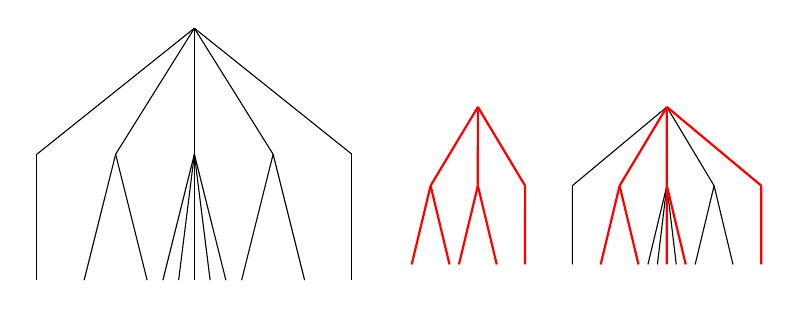
\begin{tikzpicture}
  \begin{scope}[xscale=1,yscale=1.6]
  \path (0,0) node[coordinate] (root) {};
  \foreach \x in {-2,...,2}
    {\draw (root) -- (\x,-1) node[coordinate] (n\x) {};}
  \foreach \s/\x/\n in {-2/-2/,
    -1/-1.4/,-1/-.6/,
    0/-.4/,0/-.2/,0/0/,0/.2/,0/.4/,
    1/.6/,1/1.4/,
    2/2/}
    {\draw (n\s) -- (\x,-2) node[below] {$\n$};}
  \end{scope}

  \begin{scope}[xscale=.6,yscale=1]
  \path (6,-1) node[coordinate] (root) {};
  \foreach \x in {-1,0,1}
    {\draw[red, thick] (root) -- (6+\x,-2) node[coordinate] (m\x) {};}
  \foreach \s/\x in {-1/-1.4,
				    -1/-.6,
				    0/-.4,
				    0/.4,
				    1/1}
    {\draw[red, thick] (m\s) -- (6+\x,-3);}

  \path (10,-1) node[coordinate] (root) {};
  \foreach \x in {-2,1}
    {\draw (root) -- (10+\x,-2) node[coordinate] (o\x) {};}
  \foreach \x in {-1,0,2}
    {\draw[red, thick] (root) -- (10+\x,-2) node[coordinate] (o\x) {};}
  \foreach \s/\x in {-2/-2,
			    0/-.4,
			    0/-.2,
			    0/.2,
			    1/.6,
			    1/1.4}
    {\draw (o\s) -- (10+\x,-3);}
  \foreach \s/\x in {-1/-1.4,
    			-1/-.6,
			    0/0,
			    0/.4,
			    2/2}
    {\draw[red, thick] (o\s) -- (10+\x,-3);}
  \end{scope}
\end{tikzpicture}
\caption{On the left, a tree for $d = 4$, which is the smallest $(5,2)$-universal tree:
it has size $11$ (meaning it has $11$ branches).
On the right, a tree of size $5$ and one possible embedding into the universal tree.}
\label{3-fig:example_universal}
\end{figure*}

We say that a tree $t$ embeds into another tree $T$ if:
\begin{itemize}
	\item either both are leaves,
	\item or let $t = [t_1,\dots,t_k]$ and $T = [T_1,\dots,T_{k'}]$, 
	there exist $i_1 < \dots < i_k$ such that for all $j \in [1,k]$ we have that $t_j$ embeds into $T_{i_j}$.
\end{itemize}

\begin{definition}
A tree is $(n,h)$-\textit{universal} if it embeds all trees of size $n$ and height $h$.
\end{definition}

We refer to \cref{3-fig:example_universal} for an example of a $(5,2)$-universal tree.
A first example of an $(n,h)$-universal tree is the tree where each node has degree $n$:
formally we define it recursively by $T_{n,0}$ is a leaf, and $T_{n,h+1} = [\underbrace{T_{n,h},\dots,T_{n,h}}_{n \text{ copies}}]$.
It has size $n^h$.

\subsubsection*{A quasipolynomial universal tree}
We present an inductive construction of a quasipolynomial universal tree.

\begin{theorem}
\label{3-thm:universal_tree}
There exists an $(n,h)$-universal tree with size $f(n,h)$, where $\mu$ satisfies the following:
$$\begin{array}{lll}
f(n,h) & = & f(n,h-1) + f(\lfloor n/2 \rfloor,h) + f(\lceil n/2 \rceil - 1,h), \\
f(n,1) & = & n, \\
f(1,h) & = & 1.
\end{array}$$
%Furthermore, all $(n,h)$-universal trees have size at least $g(n,h)$,
%where $\frac{f(n,h)}{g(n,h)} = O(nh)$.
\end{theorem}
An upper bound is given by
\[
f(n,h) \le 2n \binom{\lceil \log(n) \rceil + h - 1}{\lceil \log(n) \rceil}.
\]
A generous upper bound on the expression above is $n^{O(\log(h))}$.
A refined analysis reveals that the expression is polynomial in $n$ and $h$ if $h = O(\log(n))$.

%We do not prove the lower bound in this chapter.

\begin{proof}
To construct the $(n,h)$-universal tree $T$, let:
\begin{itemize}
	\item $T_\text{left}$ be a $(\lfloor n/2 \rfloor,h)$-universal tree,
	\item $T_\text{middle}$ be a $(n,h-1)$-universal tree,
	\item $T_\text{right}$ be a $(\lceil n/2 \rceil - 1,h)$-universal tree.
\end{itemize}
The intuitive construction of $T$ is as follows: 
we merge the roots of $T_\text{left}$ and $T_\text{right}$ and insert inbetween them
a child of the root to which is attached $T_\text{middle}$.
Formally, let $T_\text{left} = [T^1_{\text{left}},\dots,T^k_{\text{left}}]$ and 
$T_\text{right} = [T^1_{\text{right}},\dots,T^{k'}_{\text{right}}]$,
we define $T$ as
\[
[T^1_{\text{left}},\dots,T^k_{\text{left}},\ T_\text{middle},\ T^1_{\text{right}},\dots,T^{k'}_{\text{right}}].
\]
The construction is illustrated in \cref{3-fig:smallest_tree_construction}.

\begin{figure}[!ht]
\centering
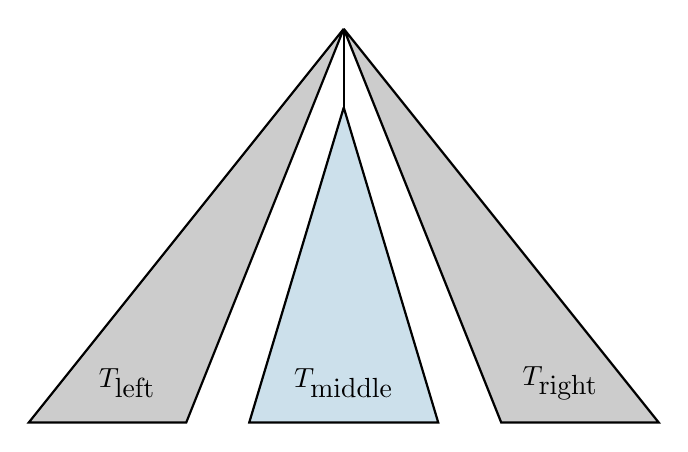
\begin{tikzpicture}
  \begin{scope}[line width=.8pt]
  \foreach \sign/\dir in {-/left,/right}
    {\draw[fill=black!20!white] (0,0) -- (\sign 4,-5) -- (\sign 2,-5) -- (0,0);
     \path (\sign 2.75,-4.5) node {$T_{\textup{\dir}}$};}
  \draw[fill=blue!60!green!20!white] (0,-1) -- (-1.2,-5) -- (1.2,-5) -- (0,-1);
  \path (0,-4.5) node {$T_{\textup{middle}}$};
  \draw (0,0) -- (0,-1);
  \end{scope}
\end{tikzpicture}
\caption{The inductive construction.}
\label{3-fig:smallest_tree_construction}
\end{figure}

\vskip1em
We argue that $T$ is $(n,h)$-universal.
Consider a tree $t = [t_1,\dots,t_k]$ with $n$ branches.
The question is where to cut, \textit{i.e.} which subtree of $t$ gets mapped to $T_\text{middle}$.
Let $n(t_i)$ be the number of branches in $t_i$. 
Since $t$ has $n$ branches, we have $n(t_1) + \cdots + n(t_k) = n$.
There exists a unique $p \in [1,k]$ such that 
$n(t_1) + \cdots + n(t_{p-1}) \le \lfloor n/2 \rfloor
\text{ and } 
n(t_1) + \cdots + n(t_p) > \lfloor n/2 \rfloor$.
The choice of $p$ implies that $n(t_{p+1}) + \cdots + n(t_k) \le \lceil n/2 \rceil - 1$.
To embed $t$ into $T$, we proceed as follows:
\begin{itemize}
	\item the tree $[t_1,\dots,t_{p-1}]$ has at most $\lfloor n/2 \rfloor$ branches,
	so it embeds into $T_\text{left}$ by induction hypothesis;
	\item the tree $t_p$ has height $h-1$ and at most $n$ branches, so in embeds into $T_\text{middle}$ by induction hypothesis;
	\item the tree $[t_{p+1},\dots,t_k]$ has at most $\lceil n/2 \rceil - 1$ branches,
	so it embeds into $T_\text{right}$ by induction hypothesis.
\end{itemize}
\end{proof}
\noindent The construction given in the proof yields the smallest $(5,2)$-universal tree illustrated in \Cref{3-fig:example_universal}.

\subsubsection*{Ordering the branches}
Let us consider a tree $t$.
A branch is given by a list of directions that we define now.
For technical convenience that will manifest itself later, the list of directions is indexed by odd numbers $p \in [1,d]$ downwards:
for example for $d = 10$ a branch is $(D_9,D_7,D_5,D_3,D_1)$.
We often naturally identify a leaf, its branch, and the list of directions that represents it.

We write $B_t$ for the set of branches of $t$ and $\le$ for the lexicographic order on $B_t$.
Note that its interpretation on the tree is: for two branches $b,b'$, we have $b \le b'$ if and only if $b$ is to the left of $b'$.
The strict version of $\le$ is $<$.

We introduce a set of relations $\vartriangleleft_p$ over $B_t$ for each $p \in [1,d]$.
For a branch $b = (D_{d-1},\dots,D_3,D_1)$ we write $b_{\ge p}$ for the tuple $(D_{d-1},\dots,D_{p+2},D_p)$,
which we call the $p$-truncated branch of $b$.
\begin{itemize}
	\item For $p$ odd, we say that $b \vartriangleleft_p b'$ 
	if $b_{\ge p}\ <\ b'_{\ge p}$.
	\item For $p$ even, we say that $b \vartriangleleft_p b'$ 
	if $b_{\ge p}\ \le\ b'_{\ge p}$.
\end{itemize}

To interpret $\vartriangleleft_p$ on the tree, we label the levels by priorities from bottom to top as in \Cref{3-fig:example_universal}.
Then $b \vartriangleleft_p b'$ if and only if the $p$-truncated branch of $b$ is to the left of the $p$-truncated branch of $b'$,
strictly if $p$ is odd, and non-strictly if $p$ is even.

\begin{figure*}[!ht]
\centering
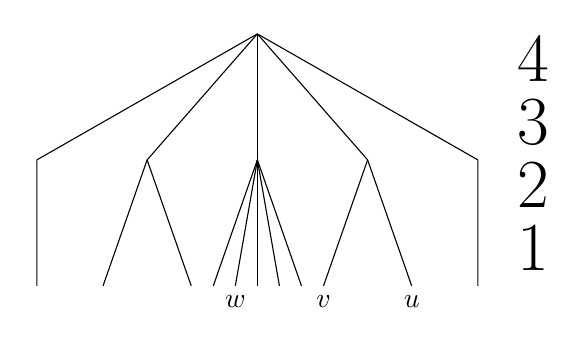
\begin{tikzpicture}
  \begin{scope}[xscale=1.4,yscale=1.6]
  \path (0,0) node[coordinate] (root) {};
  \foreach \x in {-2,...,2}
    {\draw (root) -- (\x,-1) node[coordinate] (n\x) {};}
  \foreach \s/\x/\n in {-2/-2/,
    -1/-1.4/,-1/-.6/,
    0/-.4/,0/-.2/w,0/0/,0/.2/,0/.4/,
    1/.6/v,1/1.4/u,
    2/2/}
    {\draw (n\s) -- (\x,-2) node[below] {$\n$};}
  \foreach \y/\l in {0.2/4,.7/3,1.2/2,1.7/1}
    {\draw (2.5,-\y) node {\begin{Huge}\l\end{Huge}};}
  \end{scope}
\end{tikzpicture}
\caption{Illustration of the relations $\vartriangleleft_p$.}
\label{3-fig:example_relations}
\end{figure*}

We refer to \cref{3-fig:example_relations} for some examples:
\[
v \vartriangleleft_1 u \quad ; \quad  
v \vartriangleleft_2 u \quad ; \quad 
u \vartriangleleft_2 v \quad ; \quad 
w \vartriangleleft_3 u \quad ; \quad 
w \vartriangleleft_2 v.
\]

\begin{lemma}
\label{3-lem:properties_tree}
The relations $\vartriangleleft_p$ for $p \in [1,d]$ induced by a tree $t$ satisfy the following properties:
\begin{itemize}
	\item $\vartriangleleft_d$ is the full relation: for all $b,b'$ we have $b \vartriangleleft_d b'$;
	\item if $b \vartriangleleft_p b'$ and $b' \vartriangleleft_q b''$ then $b \vartriangleleft_{\max(p,q)} b''$;
	\item the relation $\vartriangleleft_p$ is non-reflexive if $p$ is odd;
	\item the relation $\vartriangleleft_1$ is total;
	\item for $p < d$ even we have $b \vartriangleleft_p b'$ if and only if $\neg (b' \vartriangleleft_{p+1} b)$.
\end{itemize}
%Conversely, for any set of relations $\vartriangleleft_p$ for $p \in [1,d]$ over some set $V$ of size $n$ satisfying the properties above,
%there exists a tree $t$ using $V$ as set of leaves inducing these relations.
\end{lemma}
%\begin{proof}
%It is clear that the relations $\vartriangleleft_p$ induced by a tree satisfy the properties.
%
%Conversely, we give an inductive construction.
%Let us assume that the relations $\vartriangleleft_p$ are over the set $V$ of size $n$.
%At any given point we are considering a subset $S$ of $V$ and an odd priority $p$, 
%initially the whole set $V$ and the priority $d-1$.
%Given $S$ and $p$, we partition $S$ as follows:
%$S_1$ is the set of minimal elements from $S$ with respect to $\vartriangleleft_p$, 
%then $S_2$ the set of minimal elements from $S \setminus S_1$ with respect to $\vartriangleleft_p$,
%and so on: $S_k$ is the set of minimal elements from $S \setminus \bigcup_{j < k} S_j$ with respect to $\vartriangleleft_p$.
%We inductively construct the trees associated to each $S_i$ and $p-2$, yielding the tree for $S$ and $p$.
%The fact that the relation $\vartriangleleft_1$ is total implies that the leaves of the tree we construct correspond to singletons of $V$,
%hence can be identified with $V$.
%\end{proof}

The following observation rephrases the notion of embeddings between trees using the ordering on branches.

\begin{fact}
\label{3-fact:embedding}
Let $t,T$ be two trees.
Then $t$ embeds into $T$ if and only if there exists a function $\mu : B_t \to B_T$
such that for all branches $b,b'$:
\[
b \vartriangleleft_p^t b' \implies \mu(b) \vartriangleleft_p^T \mu(b').
\]
\end{fact}

\subsubsection*{Progress measures}
We explain how a tree $t$ induces both a lattice $(Y_t,\le)$ and a monotonic function $\delta_t : Y_t \times [1,d] \to Y_t$.
The set $Y_t$ is the set of branches of $t$ augmented with a new element $\bot$, 
and $\le$ is the lexicographic order on branches with $\bot$ as least element.
For each $p \in [1,d]$ and $b \in Y_t$ we extend $\vartriangleleft_p$ with $\bot \vartriangleleft_p b$.
We then define $\delta : Y_t \times [1,d] \to Y_t$ by
\[
\delta(b,p) = \max \set{b' : b' \vartriangleleft_p b}.
\]
This in turn induces a monotonic operator $\Op_t : F_V \to F_V$ defined by:
\[
\Op(\mu)(v) = 
\begin{cases}
\max \set{\delta( \mu(v'), \col(v)) : (v,v') \in E} & \text{ if } v \in \VE, \\
\min \set{\delta( \mu(v'), \col(v)) : (v,v') \in E} & \text{ if } v \in \VA.
\end{cases}
\]

Let $\Game$ be a parity game, a progress measure is a function $\mu : V \to Y_t$ which is a post-fixed point: $\mu \le \Op_t(\mu)$. 
Expanding the definitions, this means that for all vertices $v$, we have
\[
\begin{array}{llll}
\exists (v,v') \in E,\ & \mu(v) \le \delta_t( \mu(v'), \col(v)) & \text{ if } v \in \VE, \\
\forall (v,v') \in E,\ & \mu(v) \le \delta_t( \mu(v'), \col(v)) & \text{ if } v \in \VA.
\end{array}
\]
The definition of $\delta_t$ further simplifies it to: for all vertices $v$, we have
\[
\begin{array}{llll}
\exists (v,v') \in E,\ & \mu(v) \vartriangleleft_{\col(v)} \mu(v') & \text{ if } v \in \VE, \\
\forall (v,v') \in E,\ & \mu(v) \vartriangleleft_{\col(v)} \mu(v') & \text{ if } v \in \VA.
\end{array}
\]

The following theorem is our first and main step towards proving the characterisation principle.

\begin{theorem}
\label{3-thm:progress_measure}
Let $\Game$ be a parity game and $v$ a vertex.
Then Eve wins from $v$ if and only if there exists a tree $t$ and a progress measure $\mu : V \to Y_t$ such that $\mu(v) \neq \bot$.
\end{theorem}

In order to prove \cref{3-thm:progress_measure}, we first consider the case of parity graphs.
A progress measure in a parity graph is a function $\mu : V \to Y_t$ such that 
for all edges $(v,v') \in E$ we have $\mu(v) \vartriangleleft_{\col(v)} \mu(v')$.

Recall that a graph satisfies parity from $v$ if all infinite paths from $v$ satisfy parity.
This is equivalent to asking whether all cycles reachable from $v$ are even, meaning the maximal priority appearing in the cycle is even.

\begin{lemma}
\label{3-lem:progress_measure}
Let $G$ be a parity graph and $v$ a vertex.
Then $G$ satisfies parity from $v$ if and only if 
there exists a tree $t$ and a progress measure $\mu : V \to Y_t$ such that $\mu(v) \neq \bot$.
\end{lemma}

\begin{proof}
Let us assume that there exists a tree $t$ and a progress measure $\mu : V \to Y_t$ such that $\mu(v) \neq \bot$
and for all edges $(v,v') \in E$ we have $\mu(v) \vartriangleleft_{\col(v)} \mu(v')$.
To show that $G$ satisfies parity from $v$ we show that any cycle reachable from $v$ is even.
Let us consider such a cycle:
\[
(v_1,v_2) (v_2,v_3) \cdots (v_k,v_1).
\]
Since the cycle is reachable from $v$ and $\mu(v) \neq \bot$, this implies that $\mu(v_i) \neq \bot$ for $i \in [1,k]$.
Let us assume towards contradiction that its maximal priority is odd, and without loss of generality it is $\col(v_1)$.
Applying our hypothesis to each edge of the cycle we have
\[
\mu(v_1) \vartriangleleft_{\col(v_1)} \mu(v_2) \vartriangleleft_{\col(v_2)} \cdots 
\vartriangleleft_{\col(v_{k-1})} \mu(v_k) \vartriangleleft_{\col(v_k)} \mu(v_1).
\]
The second item of \cref{3-lem:properties_tree} implies that $\mu(v_1) \vartriangleleft_{\col(v_1)} \mu(v_1)$, 
which contradicts the third item since $\vartriangleleft_{\col(v_1)}$ is non-reflexive given that $\col(v_1)$ is odd.

\vskip1em
Let us now prove the converse implication.
We prove the following property by induction on the number of vertices:
for all graphs satisfying parity (without the usual assumption that every vertex has an outgoing edge),
there exists a tree $t$ and a progress measure $\mu : V \to Y_t$ such that $\mu(v) \neq \bot$
for all vertices~$v \in V$.

There are two cases: either the largest priority $d$ in the graph is even or it is odd.
We write $V_d$ for the set of vertices of priority $d$. 

\vskip1em
\textit{Case $d$ even.}
Let us consider the graph induced by the set of vertices $V \setminus V_d$.
It satisfies parity, so by induction hypothesis there exists a tree $t$ and a progress measure $\mu_d : V \setminus V_d \to Y_t$ 
such that $\mu_d(v) \neq \bot$ for all vertices $v \in V \setminus V_d$.
We extend $\mu_d$ to $\mu : V \to Y_t$: for $v \in V_d$ we let $\mu(v) = \ell_{\max}$ where $\ell_{\max}$ is the maximal element in $Y_t$.
Then $\mu$ is a progress measure such that $\mu_d(v) \neq \bot$ for all vertices $v \in V$.
Indeed the additional edges are of the form $(v,v')$ for either $v \in V_d$ or $v' \in V_d$:
in the first case $\mu(v) \vartriangleleft_{\col(v)} \mu(v')$ holds because $\vartriangleleft_d$ is the full relation,
and in the second case because $\mu(v') = \ell_{\max}$.

\vskip1em
\textit{Case $d$ odd.}
We claim that there exists a non-trivial partition $V = W_1 \uplus W_2$ such that there is no edge from $W_1$ to $W_2$.
Let $u \in V_d$, define $U$ the set of vertices reachable from $u$ by a non-trivial path.
If $U$ is empty, then $V = \set{u} \uplus (V \setminus \set{u})$ is a non-trivial partition as desired.
Otherwise $U$ is non empty, then $V = U \uplus (V \setminus U)$ is a non-trivial partition as desired:
to see that $V \setminus U$ is non empty we note that $u \in V \setminus U$, otherwise there would be an odd cycle 
(containing the maximal and odd priority $d$).

We consider the graphs induced by $W_1$ and $W_2$.
They both satisfy parity, so by induction hypothesis for $i \in \set{1,2}$ 
there exists a tree $t_i$ and a progress measure $\mu_i : W_i \to Y_{t_i}$ 
such that $\mu_i(v) \neq \bot$ for all vertices $v \in W_i$.
We let $t$ denote the tree obtained by putting the two trees $t_1$ and $t_2$ side by side with $t_2$ on the left of $t_1$.
Formally, $t_1 = [t^1_1,\dots,t^k_1]$ and $t_2 = [t^1_2,\dots,t^{k'}_2]$, let 
$t = [t^1_2,\dots,t^{k'}_2,\ t^1_1,\dots,t^k_1]$.
We define $\mu : V \to Y_t$ by $\mu(v) = \mu_i(v)$ if $v \in W_i$.
Then $\mu$ is a progress measure: for edges in the graphs induced by $W_1$ and $W_2$ this is because $\mu_1$ and $\mu_2$ are,
and the additional edges are from $v \in W_2$ to $v' \in W_1$, so indeed $\mu(v) \vartriangleleft_{\col(v)} \mu(v')$ holds.
This finishes the inductive proof of the property.

\vskip1em
We show that the property extends to graphs not satisfying parity.
Let $G$ a parity graph and $W$ the set of vertices $v$ such that $G$ satisfies parity from $v$.
Let $G'$ the graph induced by $W$, it satisfies parity so 
by the property above there exists a tree $t$ and a progress measure $\mu_W : W \to Y_t$ such that
$\mu_W(v) \neq \bot$ for all vertices $v \in W$.
We extend $\mu_W$ to $\mu : V \to Y_t$: for $v \notin W$ we let $\mu(v) = \bot$.
To see that $\mu$ is a progress measure we make two remarks.
First, if $v \in W$ then all successors of $v$ are also in $W$ (by prefix independence of parity),
so the edges in $G$ are either in $G'$ or from $v \in V \setminus W$ to $v' \in W$.
In the first case $\mu(v) \vartriangleleft_{\col(v)} \mu(v')$ holds because $\mu_W$ is a progress measure,
and in the second case because $\mu(v) = \bot$.
\end{proof}

We can now prove \cref{3-thm:progress_measure}.

\begin{proof}
Assume that Eve wins from $v$ and let $\sigma$ be a positional strategy.
The parity graph $\Game[\sigma]$ satisfies parity from $v$, so thanks to \cref{3-lem:progress_measure}
there exists a tree $t$ and a function $\mu : V \to Y_t$ such that $\mu(v) \neq \bot$
and for all edges $(v,v') \in E$ we have $\mu(v) \vartriangleleft_{\col(v)} \mu(v')$.
We remark that $\mu : V \to Y_t$ is actually a progress measure: the condition for $v \in \VE$ is ensured by the edge $\sigma(v)$,
and the condition for $v \in \VA$ by assumption on $\mu$.

\vskip1em
Conversely, assume that there exists a tree $t$ and a progress measure $\mu : V \to Y_t$.
It induces a positional strategy defined by $\sigma(v) = (v,v')$ such that $\mu(v) \vartriangleleft_{\col(v)} \mu(v')$.
We argue that $\sigma$ is a winning strategy from any vertex $v$ such that $\mu(v) \neq \bot$.
This is a consequence of \cref{3-lem:progress_measure} for the parity graph $\Game[\sigma]$.
\end{proof}

\Cref{3-thm:progress_measure} is very close to the characterisation principle we are after,
the only difference being that the lattice $(Y_t,\le)$ depends on an existentially quantified tree $t$.
This is where we use universal trees:

\begin{corollary}
\label{3-cor:progress_measure}
Let $\Game$ be a parity game with $n$ vertices and priorities in $[1,d]$, and $v$ a vertex.
Let $T$ be a $(n,d/2)$-universal tree.
Then Eve wins from $v$ if and only if there exists a progress measure $\mu : V \to Y_T$ such that $\mu(v) \neq \bot$.
\end{corollary}

\begin{proof}
Assume that Eve wins from $v$, thanks to \cref{3-thm:progress_measure} there exists a tree $t$ and a progress measure $\mu : V \to Y_t$ 
such that $\mu(v) \neq \bot$.
Since $T$ is $(n,d/2)$-universal and~$t$ has at most $n$ branches, $t$ embeds into $T$,
which thanks to \cref{3-fact:embedding} implies that there exists $\mu' : B_t \to B_T$ respecting the relations $\vartriangleleft$.
We extend it to $\mu' : Y_t \to Y_T$ by $\mu'(\bot) = \bot$.
Then the composition $\mu' \circ \mu : V \to Y_T$ is a progress measure such that $(\mu' \circ \mu)(v) \neq \bot$. 

The converse implication is a direct consequence of \cref{3-thm:progress_measure}.
\end{proof}

We have proved that the characterisation principle holds for any $(n,d/2)$-universal tree.

\subsection*{The algorithm}
Let us fix $T$ an $(n,d/2)$-universal tree.
It induces both a lattice $(Y_T,\le)$ and a monotonic function $\delta_T : Y_T \times [1,d] \to Y_T$,
which in turn induces a monotonic operator $\Op_T : F_V \to F_V$.
Since $T$ is fixed we do not specify the subscript $T$ for all these objects.

%Thanks to \cref{3-cor:progress_measure} the characterisation principle holds:
%Eve wins from $v$ if and only if there exists a progress measure $\mu : V \to Y$ such that $\mu(v) \neq \bot$.

The last step is to construct an algorithm returning the maximal progress measure relying on Kleene's fixed point theorem (stated as \cref{1-thm:kleene}).
The generic algorithm is explained in \cref{1-sec:value_iteration}, let us instantiate it here.

For the complexity analysis it is useful to decompose $\Op$ into a set of operators:
\[
\Op_v(\mu)(u) = 
\begin{cases}
\mu(v) & \text{ if } u \neq v, \\
\max \set{\delta( \mu(v'), \col(v)) : (v,v') \in E} & \text{ if } u = v \in \VE, \\
\min \set{\delta( \mu(v'), \col(v)) : (v,v') \in E} & \text{ if } u = v \in \VA.
\end{cases}
\]

We introduce some terminology: we say that an edge $e = (v,v')$ is \textit{neglected} if $\neg (\mu(v) \vartriangleleft_{\col(v)} \mu(v'))$,
and a vertex $v$ is \textit{neglected} if $\neg (\mu(v) \le \Op_v(\mu)(v))$.

\begin{figure}[!ht]
\centering
\begin{tikzpicture}
  \node[s-adam] (v) at (0,-2) {$\begin{array}{c} v \\ 3 \end{array}$};
  \node[s-eve] (v') at (2,-1) {$v'$};
  \node[s-eve] (v'') at (2,-3) {$v''$};    

    \path[arrow]
      (v) edge (v')
      (v) edge (v'');

  \begin{scope}[xscale=1.4,yscale=1.6]
  \path (5,0) node[coordinate] (root) {};
  \foreach \x in {-2,...,2}
    {\draw (root) -- (5+\x,-1) node[coordinate] (n\x) {};}
  \foreach \s/\x/\n in {-2/-2/,
    -1/-1.4/,-1/-.6/\Op_v(v),
    0/-.4/,0/-.2/,0/0/,0/.2/v'',0/.4/,
    1/.6/v',1/1.4/,
    2/2/v}
    {\draw (n\s) -- (5+\x,-2) node[below] {$\n$};}

  \node (old) at (5+2,-2.25) {};    
  \node (new) at (5-.6,-2.25) {};    
  \path[arrow]
    (old) edge[bend left, red, thick] (new);

  \foreach \y/\l in {0.2/4,.7/3,1.2/2,1.7/1}
    {\draw (7.5,-\y) node {\begin{Huge}\l\end{Huge}};}
  \end{scope}
\end{tikzpicture}
\caption{The operator $\Op_v$ in action: $\Op_v(\mu)(v)$ is the maximal leaf (meaning the rightmost leaf) 
which satisfies $\Op_v(\mu)(v) \vartriangleleft_3 \mu(v')$ and $\Op_v(\mu)(v) \vartriangleleft_3 \mu(v'')$.}
\label{3-fig:lifting}
\end{figure}

The pseudocode for the algorithm is given in \cref{3-algo:value_iteration}, 
where we let $\ell_{\max}$ denote the maximal leaf in $T$.

\begin{algorithm}[ht]
 \KwData{A parity game with $n$ vertices priorities in $[1,d]$ and a $(n,d/2)$-universal tree $T$.}
 \DontPrintSemicolon

\For{$v \in V$}{
$\mu(v) \leftarrow \ell_{\max}$
}
     
\Repeat{$\forall v \in V,\ \mu \le \Op_v(\mu)$}{
Choose $v \in V$ which is neglected

$\mu \leftarrow \min(\mu, \Op_v(\mu))$}

\Return{$\mu$}
\caption{The value iteration algorithm.}
\label{3-algo:value_iteration}
\end{algorithm}

\begin{theorem}
For all $(n, d/2)$-universal tree $T$, for all parity games $\game$ with $n$ vertices and priorities in $[1,d]$,
the value iteration algorithm over the tree $T$ returns the maximal progress measure $\mu$ for $\game$ over $T$.
\end{theorem}

Thanks to \cref{3-cor:progress_measure}, the maximal progress measure yields a solution for parity games:
Eve wins from $v$ if and only if $\mu(v) \neq \bot$.

\subsection*{Complexity analysis}
The number of times the operator $\Op_v$ is used is bounded by the number of leaves of $T$,
which we write $|T|$, implying that the total number of iterations is bounded by~$n \cdot |T|$.
%This bound cannot be much improved: for instance a vertex of priority $1$ with a self loop is evidently losing but the algorithm
%will use $|T|$ times $\Op_v$ to get this information.
To determine the overall complexity we need to discuss two aspects of the algorithm:
\begin{itemize}
	\item the data structure and in particular the choice of the vertex $v$ in the loop;
	\item the computation of $\Op_v$ and in particular the encoding of branches of $T$.
\end{itemize}

We note that a vertex $v \in \VE$ is neglected if and only if all its outgoing edges are neglected,
and a vertex $v \in \VA$ is neglected if and only if it has a neglected outgoing edge.
Hence checking whether a vertex $v$ is neglected requires considering all of its outgoing edges $(v,v')$
and checking whether $\mu(v) \vartriangleleft_{\col(v)} \mu(v')$.
Let us write $\Delta$ for the complexity of checking whether $\mu(v) \vartriangleleft_{\col(v)} \mu(v')$.
Hence checking whether $v$ is neglected costs 
$O(|\Ing^{-1}(v)| \cdot \Delta)$, where $|\Ing^{-1}(v)|$ is the number of outgoing edges of $v$.

A naive implementation of \cref{3-algo:value_iteration} would in each repeat loop go through every vertex $v$ 
to check whether it is neglected.
This would incur a linear cost: $\sum_{v \in V} O(|\Ing^{-1}(v)| \cdot \Delta) = O(m \cdot \Delta)$.
Thus the overall complexity would be
\[
O((m \cdot \Delta) \cdot (n \cdot |T|)) = O(nm \cdot \Delta \cdot |T|).
\]
Typically $\Delta$ is small (we will see that for a well chosen universal tree $T$ it is polylogarithmic in $n$ and $d$),
and $T$ is the dominating factor (quasipolynomial in $n$ and $d$ thanks to \cref{3-thm:universal_tree}).

We first explain that using a better data structure we can maintain the list of vertices $v$ such that $\neg (\mu \le \Op_v(\mu))$,
saving a linear factor in the complexity.
We then discuss the cost $\Delta$ by choosing an appropriate encoding of the quasipolynomial universal tree constructed in~\cref{3-thm:universal_tree}.

\subsubsection*{Data structure}
We use a data structure similar to the attractor computation presented in \cref{2-sec:attractors}.
The pseudocode is given in \cref{3-algo:value_iteration_data_structure}.
We did not provide the pseudocode for the functions $\texttt{Init}$ and $\texttt{Update}$.

The data structure consists of the following objects:
\begin{itemize}
	\item a leaf of $T$ for each vertex, representing the current function $\mu : V \to Y$;
	\item a set $S$ of vertices (each vertex appears at most once in $S$, the order in which vertices are stored and retrieved from the set does not matter);
	\item for each vertex of Eve a number of edges.
\end{itemize}
For our complexity analysis we use the unit cost RAM model, see \cref{1-sec:computation} for details.
In the case at hand let us choose for the machine word size $w = \log(m) + \log(d)$, 
so that an edge together with its priority can be stored in one machine word.
The space complexity of this data structure depends on the encoding of $T$, which we will discuss later.

The invariant of the algorithm satisfied before each iteration of the repeat loop is the following:
\begin{itemize}
	\item for $v \in \VA$, the value of $\text{number}$-$\text{neglected}$-$\text{edges}(v)$
	is the number of neglected edges of $v$;
	\item $S$ is the set of neglected vertices.
\end{itemize}
The invariant is satisfied initially thanks to the function $\texttt{Init}$.
Let us assume that we choose and remove $v$ from $S$.
Since we modify only $\mu(v)$ the only potentially neglected vertices are in $S$ (minus $v$) and the incoming edges of $v$;
for the latter each of them is checked and added to $S$ when required.
By monotonicity, neglected vertices remain neglected so all vertices in $S$ (minus $v$) are still neglected.
Hence the invariant is satisfied.

The invariant implies that the algorithm indeed implements~\cref{3-algo:value_iteration} hence returns the maximal progress measure, 
but it also has implications on the complexity.
Indeed one iteration of the repeat loop over some vertex $v$ involves 
\[
O\left( (|\Ing^{-1}(v)| + |\Out^{-1}(v)|) \cdot \Delta \right)
\]
operations,
the first term corresponds to updating $\mu(v)$ and $\text{number}$-$\text{neglected}$-$\text{edges}(v)$,
which requires for each outgoing edge of $v$ to compute $\delta$,
and the second term corresponds to considering all incoming edges of $v$ and treating the neglected ones.
Thus the overall complexity is
\[
O\left( 
\sum_{v \in V} (|\Ing^{-1}(v)| + |\Out^{-1}(v)|) \cdot \Delta \cdot |T|
\right) 
= O(m \cdot \Delta \cdot |T|).
\]

\begin{algorithm}
 \KwData{A parity game with $n$ vertices priorities in $[1,d]$ and a $(n,d/2)$-universal tree $T$.}
 \SetKwFunction{FTreat}{Treat}
 \SetKwFunction{FVI}{ValueIteration}
 \SetKwFunction{FInit}{Initialise}
 \SetKwFunction{FUpdate}{Update}
 \SetKwProg{Fn}{Function}{:}{}
 \DontPrintSemicolon
 
\Fn{\FVI{}}{
%	\For{$v \in V$}{
%		$\mu(v) \leftarrow \ell_{\max}$
%	}
	
	\FInit{$\mu$, $\text{number}$-$\text{neglected}$-$\text{edges}$, $S$}

%	\vskip1em
%	\For{$e \in E$}{	
%		\If{$e$ is neglected}{
%			\FTreat($e$)
%		}
%	}

	\vskip1em
	\Repeat{$S$ empty}{
		Choose some $v$ in $S$ and remove it from $S$

		$\mu \leftarrow \min(\mu, \Op_v(\mu))$

		\FUpdate{$\text{number}$-$\text{neglected}$-$\text{edges}(v)$}

		\For{$e \in E$ \text{ such that } $\Out(e) = v$}{
			\If{$e$ is neglected}{
				\FTreat($e$)
			}
		}
	}

	\Return{$\mu$}
}

\vskip1em
\Fn{\FTreat{$e$}}{
	$v \leftarrow \Ing(e)$
	
	\If{$v \in \VA$ and $v \notin S$}{
		Add $v$ to $S$		
	}
	
	\If{$v \in \VE$ and $v \notin S$}{	
		$\text{number}$-$\text{neglected}$-$\text{edges}(v) \leftarrow \text{number}$-$\text{neglected}$-$\text{edges}(v) + 1$

		\If{$\text{number}$-$\text{neglected}$-$\text{edges}(v) = $ number of outgoing edges of $v$}{
			Add $v$ to $S$
		}
	}
}
\caption{The value iteration algorithm with explicit data structure.}
\label{3-algo:value_iteration_data_structure}
\end{algorithm}

\subsubsection*{Encoding branches}
Let us fix $T$ to be the quasipolynomial universal tree constructed in \cref{3-thm:universal_tree}.

In our definition of trees we say that a tree is an ordered list of subtrees $[t_1,\dots,t_k]$,
so we use $[1,k]$ with the natural order for ordering the subtrees.
Any other total order can be used to that effect, and a more appropriate order may lead to smaller encoding.
Indeed, using $[1,k]$ for ordering subtrees, if a tree has height $h$ and $n$ branches then a branch is a sequence of $h$ numbers in $[1,n]$,
so it uses $O(h \log(n))$ bits.

Let us consider an order well suited for encoding $T$.
We use $\set{0,1}^*$ the set of binary words and order them using the following three rules that apply for any $u,v \in \set{0,1}^*$:
\[
0u < \varepsilon < 1u \quad ; \quad (0u < 0v \Longleftrightarrow u < v) \quad ; \quad (1u < 1v \Longleftrightarrow u < v).
\]
For words of length at most $2$ the order is $00 < 0 < 01 < \varepsilon < 10 < 1 < 11$.

\begin{figure}[!ht]
\centering
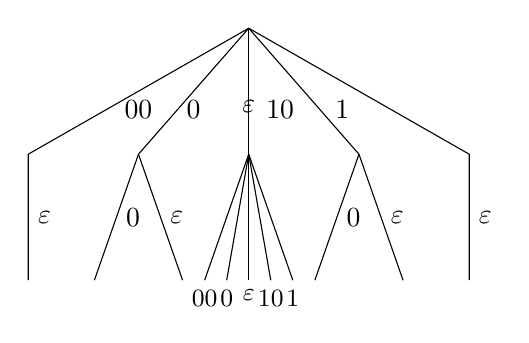
\begin{tikzpicture}
  \begin{scope}[xscale=1.4,yscale=1.6]
  \path (0,0) node[coordinate] (root) {};
  \foreach \x/\n in {-2/00,
  				-1/0,
  				0/\varepsilon}
    {\draw (root) -- node[below] {$\n$} (\x,-1) node[coordinate] (n\x) {};}
  \foreach \x/\n in {1/10,
  				2/1}
    {\draw (root) -- node[below left] {$\n$} (\x,-1) node[coordinate] (n\x) {};}

  \foreach \s/\x/\n in {-2/-2/\varepsilon,
					-1/-1.4/0,
					-1/-.6/\varepsilon,
    				1/.6/0,
    				1/1.4/\varepsilon,
    				2/2/\varepsilon}
    {\draw (n\s) -- node[right] {$\n$} (\x,-2);}
  \foreach \s/\x/\n in {0/-.4/00,
				    0/-.2/0,
				    0/0/\varepsilon,
				    0/.2/10,
				    0/.4/1}
    {\draw (n\s) -- (\x,-2) node[below] {\begin{small}$\n$\end{small}};}
  \end{scope}
\end{tikzpicture}
\caption{The succinct encoding on the $(5,2)$-universal tree.}
\label{3-fig:tree_encoded}
\end{figure}

We can now revisit the construction of the universal tree by defining directly the set of branches.
Recall that $T$ is obtained from $T_\text{left},T_\text{middle}$, and $T_\text{right}$. 
By induction hypothesis branches in $T_\text{left}$ and $T_\text{right}$ are tuples of length $h-1$
and branches in $T_\text{middle}$ tuples of length $h$.
The branches of $T$ are:
\begin{itemize}
	\item branches of $T_\text{left}$ where the first component is prefixed with a $0$;
	\item branches of $T_\text{middle}$ augmented with a new component $\varepsilon$;
	\item branches of $T_\text{right}$ where the first component is prefixed with a $1$.
\end{itemize}
We call this encoding the ""succinct encoding"", it is illustrated in \cref{3-fig:tree_encoded} for the $(5,2)$-universal tree.
The leftmost branch is $(00,\varepsilon)$, and the middle branch $(\varepsilon,\varepsilon)$.
In general, the inductive construction implies that every branch is a tuple $(D_{d-1},\dots,D_1)$ 
such that the sum of the lengths of the directions $D_i$ is at most $\log(n)$.
Thus a branch is encoded using $O(\log(h) \log(n))$ bits: for each of the $\log(n)$ bits we need $\log(h)$ bits to specify its component.

In terms of machine words of size $w = \log(n) + \log(d)$, this means that a branch can be stored using $\log(d)$ machine words.
Hence the data structure uses $O(n \log(d))$ machine words, with together with the input size $O(m)$
means that the space complexity of the algorithm is $O(m + n \log(d))$.

\vskip1em
Using the succinct encoding and a tedious but simple case analysis we can compute $\delta(b,p)$ in time $O(\log(n) \log(d))$.
Putting everything together we obtain the overall complexity 
\[
O\left(nm \log(n) \log(d) \cdot  \binom{\lceil \log(n) \rceil + d/2 - 1}{\lceil \log(n) \rceil} \right),
\]
as stated in \cref{3-thm:value_iteration_quasipoly}.


%%%%%%%%%%%%%%%%%%
%%%%%%%%%%%%%%%%%%
%%%%%%%%%%%%%%%%%%

\section{Comparing the three families of algorithms}
\label{3-sec:relationships}
At the beginning of the chapter we described three families of algorithms: 
strategy improvement, attractor decomposition, and value iterations.

\vskip1em
Let us first clarify the relationship between the separation framework discussed in \cref{3-sec:separation}
and the value iteration paradigm presented in \cref{3-sec:value_iteration}.
Both are families of algorithms: 
\begin{itemize}
	\item An $(n,d)$-separating automaton $\Automaton$ induces an algorithm for solving parity games in time 
$O(m \cdot |\Automaton|)$ where $|\Automaton|$ is the size of $\Automaton$, meaning the number of states.
	\item An $(n,d/2)$-universal tree $T$ induces a value iteration algorithm for solving parity games in time 
proportional to $|T|$ where $|T|$ is the size of $T$, meaning the number of leaves (the exact complexity depends on the cost of computing $\delta$ in $T$, which is typically small).
\end{itemize}
These two families are in a strong sense equivalent:

\begin{theorem}\hfill
\begin{itemize}
	\item An $(n,d)$-separating automaton induces an $(n,d/2)$-universal tree of the same size;
	\item An $(n,d/2)$-universal tree induces an $(n,d)$-separating automaton of the same size.
\end{itemize}
\end{theorem}
We do not prove this theorem here but note that it can be stated more generally for any positionally determined objective,
replacing universal trees by the notion of universal graphs.

The main advantage of the value iteration presentation is the space complexity, which for a good choice of the universal tree
can be made very small (quasilinear).

\vskip1em
In terms of complexity, the strategy improvement has exponential complexity, while both attractor decompositions and value iterations algorithms have quasipolynomial complexity.
Let us make a finer comparison: the complexity of the attractor decomposition algorithm is a polynomial multiplied by the (non polynomial) term
\[
\binom{\lceil \log(n) \rceil + d - 1}{\lceil \log(n) \rceil},
\]
while for the value iteration algorithm the complexity is a polynomial multiplied by the (also non polynomial) term
\[
\binom{\lceil \log(n) \rceil + d/2 - 1}{\lceil \log(n) \rceil}.
\]
The key difference is that the former performs an induction using all priorities, while the latter considers only odd priorities hence the dependence in $d/2$.
Although our presentation of the attractor decomposition algorithm does not make it explicit, 
this class of algorithms is also related to the notion of universal trees; 
however an algorithm is induced not by one $(n,d/2)$-universal tree, but by two: one for each player,
which are then interleaved to organise the recursive calls of the algorithm.

\vskip1em
Since both value iteration and attractor decomposition algorithms are connected to the combinatorial notion of universal trees,
the next question is whether the construction given in \cref{3-sec:value_iteration} is optimal.
The answer is unfortunately yes, there exists a lower bound on the size of universal trees which matches this construction up to polynomial factors.

\vskip1em
The last question we discuss here is whether there exists a quasipolynomial strategy improvement algorithm.
In particular a natural attempt would be to use universal trees for this endeavour.
Unfortunately, this fails: \cref{3-lem:key_property} explains that for the particular choice of the lattice $Y$,
functions $\mu : V \to Y$ can be used both to certify that a graph satisfies parity or that it satisfies the complement of parity.
Both implications are used in the correctness proof of the algorithm.
This symmetric feature is lost with universal trees, which only satisfy one of the two implications, stated in \cref{3-lem:progress_measure}.


%%%%%%%%%%%%%%%%%%
%%%%%%%%%%%%%%%%%%
%%%%%%%%%%%%%%%%%%

\section*{Bibliographic references}
\label{3-sec:references}
As discussed in the introduction, the literature on multiobjective models is too vast to provide a full account here. We therefore focus on some directions particularly relevant to our focus.

\paragraph{Multidimension games.} Energy games and their related work were discussed in~\cref{chap:counters}. Our presentation of mean-payoff games is inspired by Velner et al.~\cite{Velner&al:2015}. Brenguier and Raskin studied the Pareto curves of these games in~\cite{Brenguier&Raskin:2015}. While we considered \textit{conjunctions} of mean-payoff objectives, Velner proved that Boolean combinations lead to undecidability~\cite{Velner:2015}.

The undecidability of total-payoff games was first established in~\cite{Chatterjee&al:2015} via reduction from the halting problem for two-counter machines: we provided here a new, simpler proof based on robot games~\cite{Niskanen&Potapov&Reichert:2016}. This undecidability result, along with the complexity barriers of mean-payoff and total-payoff games, motivated the introduction of (multidimension) ""\textit{window objectives}"": conservative variants of mean-payoff and total-payoff objectives that benefit from increased tractability and permit to reason about time bounds~\cite{Chatterjee&al:2015}. Window variants of "parity" objectives have been studied in~\cite{Bruyere&Hautem&Randour:2016}.

\paragraph{Combinations of different objectives.} We focused on multidimension games obtained by conjunction of \textit{identical} objectives. Conjunctions of \textit{heterogeneous} objectives have been studied in a variety of contexts including mean-payoff parity games~\cite{Chatterjee&Henzinger&Jurdzinski:2005,Daviaud&Jurdzinski&Lazic:2018}, energy parity games~\cite{Chatterjee&Doyen:2012,Chatterjee&Randour&Raskin:2014}, average-energy games with energy constraints~\cite{Bouyer&al:2018,Bouyer&al:2017}, simple quantitative objectives~\cite{Bruyere&Hautem&Raskin:2016}. Le Roux, Pauly and Randour studied general conditions under which finite-memory strategies suffice to play optimally, even in a broad multi-objective setting~\cite{LeRoux&Pauly&Randour:2018}.


\paragraph{Beyond worst-case synthesis.} Our presentation is mostly based on~\cite{Bruyere&al:2017}, where all technical details can be found. As noted in~\cite{Bruyere&al:2017}, allowing large inequalities in the BWC problem may require infinite-memory strategies. The case of infinite-memory strategies was studied in~\cite{Clemente&Raskin:2015} along with multidimension BWC mean-payoff problems. BWC problems were studied for other objectives, such as shortest path~\cite{Bruyere&al:2017} or parity~\cite{Berthon&Randour&Raskin:2017}; and on other related models (e.g.,~\cite{Brazdil&Kucera&Novotny:2016,Almagor&Kupferman&Velner:2016}). BWC principles have been implemented in the tool \textsc{Uppaal}~\cite{David&al:2014}.

Comparisons with other rich behavioural models can be found in~\cite{Randour&Raskin&Sankur:2015,Brenguier&al:2016}.



